% paper/sections/12u8_time_integration.tex
%
% U8: Time-integration suite (TVD-RK3, EXT2, implicit-BDF2, layer convergence) — Tier V
% ═══════════════════════════════════════════════════════════════════════════════
\subsubsection{U8：時間積分スイート（TVD--RK3 / EXT2 / implicit-BDF2 / Layer A,B,C）[Tier V]}
\label{sec:U8_time_integration}

\paragraph{検証対象．}
第~\ref{sec:time_int}章 で導入した時間積分の全要素を単体検証する：
TVD--RK3~\cite{ShuOsher1988,JiangShu1996}（§\ref{sec:time_int}：3 次 SSP），
EXT2/AB2 形の 2 次外挿（§\ref{sec:time_level1}），
そして粘性項の \textbf{implicit-BDF2}（§\ref{sec:time_viscous}）を測る．
周期拡散 MMS では FFT 対角化した Laplacian に BDF1 起動 + BDF2 を直接適用し，
2 次精度と A--stable damping を分離して確認する．
A/B/C 3 層粘性切替（§\ref{sec:viscous_3layer}：均一 / 中濃度差 / 強濃度差）は，
現在の implicit-BDF2 + DC 契約に合わせ，full variable-viscosity operator を
同時刻で陰的に解く fixed-point limit として検証する．

\paragraph{設定．}
\begin{description}\setlength{\itemsep}{0pt}
  \item[U8-a] TVD--RK3 単体．スカラー ODE $\dot{u} = -\lambda u, \lambda=1, T=1$．
        $n_t \in \{4,8,\dots,512\}$．設計次数 3．
        production の \texttt{twophase.time\_integration.tvd\_rk3} を直接駆動．
  \item[U8-b] EXT2/AB2 単体．同 ODE．$n_t \in \{16,\dots,512\}$．設計次数 2．
        本テストは \emph{ODE ベンチマーク}（インライン textbook EXT2/AB2 を用いる）であり，
        production の \texttt{Predictor} 経路（NS 連成・FlowState/ConvectionTerm/...
        を要求）はスカラー ODE には適用不可．production と同一の EXT2 公式
        $u_{n+1} = u_n + \mathrm{d}t (\tfrac{3}{2} f_n - \tfrac{1}{2} f_{n-1})$
        を用いるため，設計次数 2 を露出する目的に対しては等価．
  \item[U8-c] implicit-BDF2 spectral 拡散方程式．$\nu = 0.01$，2D 拡散方程式，
        $n_t \in \{10,\dots,320\}$．設計次数 2．
        \textbf{安定性}：CFL$_\nu \in \{0.5,1,5,10\}$ で BDF2 は安定．
        FE は CFL$_\nu \le 1.0$ で発散（高波数モードが励起される領域）；
        CFL$_\nu \ge 5$ では smooth IC の低周波成分のみが進化するため
        見かけ上 growth $\sim 0.62$ に収まる（高周波成分の blowup は潜在）．
  \item[U8-d] A/B/C 3 層 implicit-BDF2 full-operator test（界面 viscosity ratio test, 1D MMS）．
        $\mu_{\mathrm{ratio}} \in \{10, 100\}$，layer $\in \{$A, B, C$\}$，
        $n_t \in \{16,\dots,256\}$．
        $L_{\mathrm{full}} = \partial_x(\mu \partial_x \cdot)$ を conservative face-average
        で離散化し，BDF1 起動後に BDF2 で full operator を陰的に解く．
        Layer A=均一 / B=粘性勾配 (band $1.5h$) / C=HFE 平滑化 (band $5h$)．
        MMS source は同じ離散 $L_{\mathrm{full}}$ から作るため，空間誤差を消し
        時間骨格だけを測る．
\end{description}

\paragraph{結果．}

\begin{table}[!ht]
\caption{U8-a/U8-b/U8-c：時間積分 3 単体の格子収束}
\label{tab:U8_basic_orders}
\PaperCaptionNote{TVD--RK3 slope $3.04$（設計 3），EXT2/AB2 slope $2.05$（設計 2），implicit-BDF2 spectral slope $2.01$（設計 2）．全て理論次数を達成し，U8-c は §\ref{sec:time_viscous} の BDF2 粘性骨格と対応する．}
\centering\small
\begin{tabular}{r c r c r c}
\toprule
\multicolumn{2}{c}{TVD--RK3} & \multicolumn{2}{c}{EXT2/AB2} & \multicolumn{2}{c}{implicit-BDF2} \\
\cmidrule(lr){1-2}\cmidrule(lr){3-4}\cmidrule(lr){5-6}
$n_t$ & err & $n_t$ & err & $n_t$ & err \\
\midrule
$4$   & $2.93\times 10^{-4}$ & $16$  & $1.42\times 10^{-4}$ & $10$   & $6.69\times 10^{-4}$ \\
$8$   & $3.31\times 10^{-5}$ & $32$  & $3.27\times 10^{-5}$ & $20$   & $1.65\times 10^{-4}$ \\
$16$  & $3.93\times 10^{-6}$ & $64$  & $7.84\times 10^{-6}$ & $40$   & $4.09\times 10^{-5}$ \\
$32$  & $4.80\times 10^{-7}$ & $128$ & $1.91\times 10^{-6}$ & $80$   & $1.02\times 10^{-5}$ \\
$64$  & $5.92\times 10^{-8}$ & $256$ & $4.73\times 10^{-7}$ & $160$  & $2.54\times 10^{-6}$ \\
$128$ & $7.35\times 10^{-9}$ & $512$ & $1.18\times 10^{-7}$ & $320$  & $6.35\times 10^{-7}$ \\
\midrule
slope & $\mathbf{3.04}$ & slope & $\mathbf{2.05}$ & slope & $\mathbf{2.01}$ \\
\bottomrule
\end{tabular}
\end{table}

\begin{table}[!ht]
\caption{U8-c：implicit-BDF2 spectral と FE の安定性比較}
\label{tab:U8_stability}
\PaperCaptionNote{前進 Euler (FE)，$\nu=0.01$, $T=0.5$．BDF1 起動 + implicit-BDF2 は CFL$_\nu = 10$ でも growth $\sim 0.65$ 安定；FE は CFL$_\nu = 0.5$ で $1.73\times 10^{21}$ に爆発．§\ref{sec:time_operator_stiffness} の A--stable 分類と整合．}
\centering\small
\begin{tabular}{r r r r}
\toprule
CFL$_\nu$ & $\mathrm{d}t$ & BDF2 growth & FE growth \\
\midrule
$0.5$  & $0.0122$ & $0.6409$ & $1.73\times 10^{21}$ \\
$1.0$  & $0.0244$ & $0.6410$ & $1.84\times 10^{9}$ \\
$5.0$  & $0.122$  & $0.6434$ & $0.6304$ \\
$10.0$ & $0.244$  & $0.6480$ & $0.6228$ \\
\bottomrule
\end{tabular}
\end{table}

\begin{table}[!ht]
\caption{U8-d：A/B/C 3 層 implicit-BDF2 粘性テスト}
\label{tab:U8_layers}
\PaperCaptionNote{full variable-viscosity operator を BDF1 起動 + implicit-BDF2 で陰的に解く 1D MMS（$T=0.02$）．Layer A（均一），Layer B（band $1.5h$），Layer C（band $5h$）の全ケースで 2 次を維持し，cross 項の時間遅れを導入しない現在の §\ref{sec:time_viscous} 契約と整合する．}
\centering\small
\begin{tabular}{r r r r r r}
\toprule
$n_t$ & A ($\mu\!=\!1$) & B ($\!10$) & B ($\!100$) & C ($\!10$) & C ($\!100$) \\
\midrule
$16$  & $9.61\times 10^{-7}$  & $6.31\times 10^{-7}$ & $3.82\times 10^{-7}$ & $5.90\times 10^{-7}$ & $1.84\times 10^{-7}$ \\
$32$  & $2.39\times 10^{-7}$  & $1.56\times 10^{-7}$ & $9.32\times 10^{-8}$ & $1.45\times 10^{-7}$ & $4.40\times 10^{-8}$ \\
$64$  & $5.97\times 10^{-8}$  & $3.86\times 10^{-8}$ & $2.30\times 10^{-8}$ & $3.60\times 10^{-8}$ & $1.08\times 10^{-8}$ \\
$128$ & $1.49\times 10^{-8}$  & $9.62\times 10^{-9}$ & $5.73\times 10^{-9}$ & $8.97\times 10^{-9}$ & $2.67\times 10^{-9}$ \\
$256$ & $3.72\times 10^{-9}$  & $2.40\times 10^{-9}$ & $1.43\times 10^{-9}$ & $2.24\times 10^{-9}$ & $6.64\times 10^{-10}$ \\
\midrule
slope & $\mathbf{2.00}$ & $\mathbf{2.01}$ & $\mathbf{2.02}$ & $\mathbf{2.01}$ & $\mathbf{2.03}$ \\
\bottomrule
\end{tabular}
\\[2pt]
{\footnotesize Layer B/C も $L_{\mathrm{full}}=\partial_x(\mu\partial_x\cdot)$ を同時刻で陰的に解くため，粘性勾配項は explicit cross 誤差として現れない．}
\end{table}

\begin{figure}[!ht]
\centering
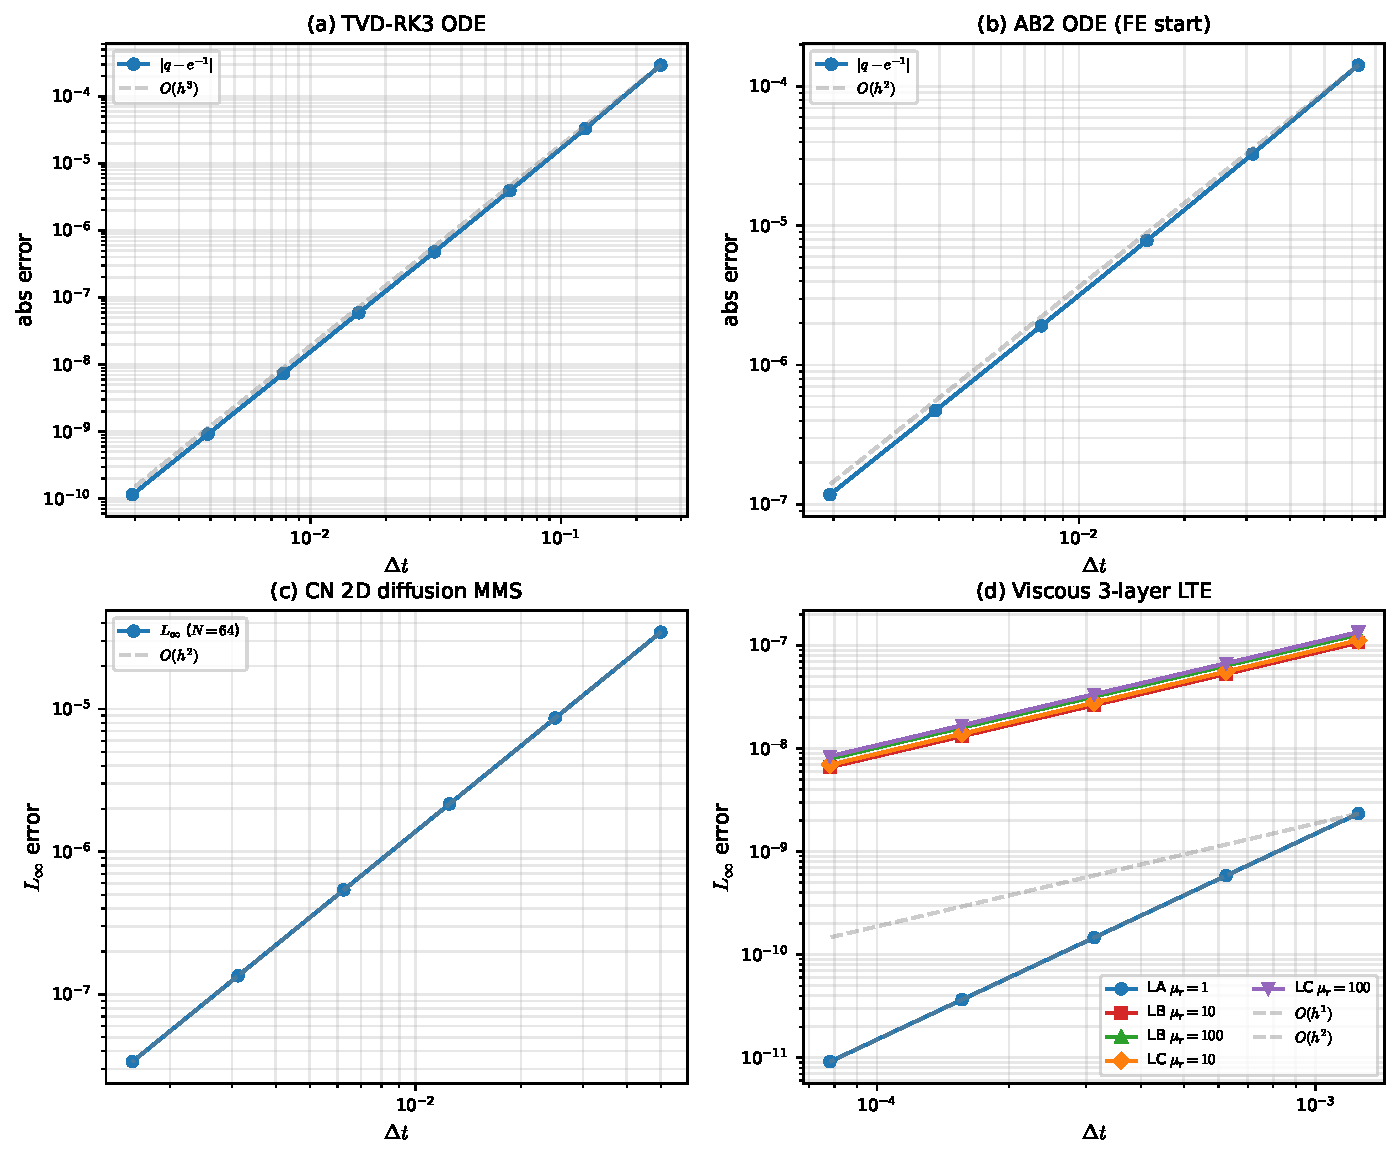
\includegraphics[width=0.88\linewidth]{figures/ch12_u8_time_integration_suite}
\caption{U8：TVD--RK3 / EXT2 / implicit-BDF2 3 種積分子}
\label{fig:ch12_u8}
\PaperCaptionNote{基本収束 slope $3.04 / 2.05 / 2.01$ で各設計次数を達成； implicit-BDF2 vs FE 安定性比較で CFL$_\nu = 0.5$ にて FE 増幅 $1.73\times 10^{21}$ 発散・BDF2 は $0.64$ 抑制； 3 層 full-operator BDF2 で Layer A/B/C 全て 2 次を維持．}
\end{figure}

\paragraph{判定と次章への接続．}
\begin{itemize}\setlength{\itemsep}{0pt}
  \item U8-a TVD--RK3：slope $3.04$，設計 3 次完全達成．\checkmark
  \item U8-b EXT2/AB2：slope $2.05$，設計 2 次完全達成．\checkmark
        $0.05$ の上振れは FE start--up step
        （EXT2/AB2 の 1 step 目の Forward--Euler 起動）に由来する $\Ord{\mathrm{d}t^2}$
        ではなく $\Ord{\mathrm{d}t^3}$ の transient であり，
        $n_t$ を増やすほど該当寄与が相対的に小さくなって観測 slope が
        設計 2 次に上から漸近する典型的挙動．許容帯
        $|p_{\mathrm{measured}} - p_{\mathrm{design}}| \le 0.5$ の十分内側．
  \item U8-c implicit-BDF2 spectral：slope $2.01$，FE 比 安定性 $\approx 21$ 桁優位
        ($\log_{10}(1.73\!\times\!10^{21}/0.6409) \approx 21.4$；CFL$_\nu=0.5$ にて)．
        §\ref{sec:time_operator_stiffness} の A--stable 分類と整合．\checkmark
  \item U8-d Layer A/B/C：full variable-viscosity operator を同時刻 implicit-BDF2 で解くと，
        A/B/C 全ケースで slope $2.00$--$2.03$ を維持する．
        これは §\ref{sec:time_viscous} の implicit-BDF2 + DC fixed-point 契約
        （cross 項を時間的に外挿せず，高次残差内で同時刻評価する）と整合する．\checkmark
\end{itemize}
検証対応：
式~\eqref{eq:tvd_rk3}（SSP 形），EXT2 multistep 公式，
implicit-BDF2 amplification factor と full variable-viscosity operator に対し，
ODE/MMS 収束と粘性安定性を測定する．
